\chapter[Recurrent Neural Networks for Timeseries Analysis]{Recurrent Neural Networks for Timeseries Analysis}\label{ch:07}

In this chapter, you'll learn about recurrent neural networks, a class of neural networks particularly suited to handle sequential data, such as timeseries and videos.

You'll start by coding a standard recurrent neural network using PyTorch. Then, you'll embed it into a Deeplay model, streamlining it for ease of use and learning how to implement your own models in Deeplay. Finally, you'll tackle real-world problems like temperature forecasting and language translation.

\section{Understanding Recurrent Neural Networks}

Unlike the neural networks you've encountered until now that treat each data sample independently, recurrent neural networks are designed to analyze data in a sequence, which is useful, for example, for analyzing timeseries and videos. 

This type of network uses \emph{recurrence relations}, mathematical operations applied to sequences in which the value of an element is determined by the preceding elements. For example, the location of an object in one frame of a movie often provides useful information about where it'll be in subsequent frames. Recurrent neural networks use a form of \emph{memory} to utilize this past history.

\subsection{Comb Filter}

To illustrate how recurrence relations work in practice, think of the task of processing a numerical sequence where the output of one step is the average of the current input and the output of the previous step. This procedure of reintroducing the output as part of the input establishes a \emph{feedback loop}. In signal processing, this technique is known as a \emph{comb filter}. For example, comb filters are used in various sound effects such as \emph{reverb} (which simulates the echoes and reflections of sound within an acoustic space), \emph{flanging} (which mixes a signal with a slightly delayed copy of itself to produce a distinctive swirling sound), and \emph{pitch shifting} (which changing the pitch of a sound without altering its duration, allowing for adjustments in musical key or tonality).

You can implement a comb filter with the code in Listing~\ref{cd:07:0}.
\begin{lstlisting}[
    label=cd:07:0,
    caption=Implementing a comb filter 
]
input_series = [0, 0, 0, 0, 1, 1, 1, 1, 1, 1, 1, 1, 0, 0, 0, 0, 0, 0, 0, 0]

state, U, V = 0, 0.5, 0.5

output_series = []
for input_data in input_series:
    (@\codewingding{1}@)hidden = U * input_data + V * state
    output_data = hidden
    state = output_data
    output_series.append(output_data)
\end{lstlisting}
This simple comb filter operates on the \lstinline{input_series} list, which corresponds to a square wave. 
The \lstinline{state} variable, which is initialized to 0 records the output at the previous step.
The \lstinline{U} constant determines the weight of the current input (\lstinline{input_data}) in the calculation, while the \lstinline{V} constant
defines the weight of the \lstinline{state} variable. Here, these variables are set so that both \lstinline{input_data} and \lstinline{state} each contributes 50 percent to the final output.

This code then iteratively applies the comb filter to each value in the input series.
Fist, it calculates the updated average by weighing the current input and the previous state, and saves it into the \lstinline{hidden} variable \wingding{1}.
Then, it sets the current output (\lstinline{output_data}) to the value of the \lstinline{hidden} variable and updates the \lstinline{state} to the value of \lstinline{output_data}. And finally, it appends \lstinline{output_data} to the \lstinline{output_series} list.

By printing the output series with
\begin{lstlisting}
print(f"Output Series: {[f'{x:.2f}' for x in output_series]}")
\end{lstlisting}
you get:
\begin{lstlisting}
Output Series: ['0.00', '0.00', '0.00', '0.00', '0.50', '0.75', '0.88', '0.94', 
'0.97', '0.98', '0.99', '1.00', '0.50', '0.25', '0.12', '0.06', '0.03', '0.02', 
'0.01', '0.00']
\end{lstlisting}
The output series slowly starts increasing when the input signal suddenly becomes equal to 1 and reaches this value after some delay. A similar behavior occurs as the input changes to 0, which causes the output to decrease to 0 over multiple steps.

\subsection{A Simple Recurrent Neural Network}

Just like in a comb filter, where the previous output is fed back as an additional input, a recurrent neural network also feeds its output back into the input. This feedback mechanism, as illustrated in Figure~\ref{fig:07:01}, enables the network to maintain a form of memory and effectively analyze sequential data.

\begin{figure}[H]
	\includegraphics[width=4.675in]{ch_07/fig_07_01} %%% THIS FIGURE WILL BE REDRAWN - CHANGE SIZE - REVISE ALSO NOTATION TO BE CONSISTENT WITH SECTION AND CODE - ALSO: add the scheme of the filter and the graph of the processed square wave
	\caption{Working principle of a recurrent neural network}
	\label{fig:07:01}
\end{figure}

On the left side of Figure~\ref{fig:07:01}, the recurrent neural network receives a value of the input series as input. Next, it transforms the input through a hidden layer, which combines the input and the previously memorized state. Then, it calculates the output through an additional layer and updates its memorized state to the value of the current output.
On the right side of Figure~\ref{fig:07:01}, the same recurrent neural network is shown unfolded in time, highlighting its sequential computation process.

You can implement this recurrent neural network by updating Listing~\ref{cd:07:0} as shown in Listing~\ref{cd:07:1}. 
\begin{lstlisting}[
	label=cd:07:1,
	caption=Implementing a recurrent neural network in NumPy
    (\expand{cd:07:0})
]
***import numpy as np

def sigmoid(x):
    """Simple implementation of sigmoid function."""
    return 1 / (1 + np.exp(-x))***

input_series = [0, 0, 0, 0, 1, 1, 1, 1, 1, 1, 1, 1, 0, 0, 0, 0, 0, 0, 0, 0]

state = 0
(@\codewingding{1}@)***U, V, W, b = np.random.normal(size=4)***

output_series = []
for input_data in input_series:
    hidden = ***sigmoid(***U * input_data + V * state ***+ (@\wingding{2}@)b)***
    output_data = ***sigmoid((@\wingding{3}@)W * ***hidden***)***
    state = output_data
    output_series.append(output_data)
\end{lstlisting}
In this code, the weights of the network are randomly initialized \wingding{1}.
As in the previous example, this code computes the \lstinline{hidden} state by combining the input and state signals, as well as by adding a bias \wingding{2}. Then, it transforms the result with a sigmoid function to introduce a non-linearity.
Finally, the code computes the output as the product of the hidden state with an output weight \wingding{3} transformed by a sigmoid function to introduce an additional non-linearity.
Of course, since this simple neural network is randomly initialized, the output series will be random.

\begin{nspbox}{Exercise}
\begin{description}
	\item[7-1: Implementing recurrent backpropagation]
    Although the previous example shows the principle behind recurrent neural networks, you can't use it to solve any concrete problem without training the weights.
    To do so, implement recurrent backpropagation and use it to train the recurrent neural network to perform some simple operations on timeseries (for example, to damp a sinusoidal wave).
    
	\item[7-2: Implement recurrent neural networks with higher-dimensional data]
    Generalize this implementation of a recurrent neural network to accept multi-dimensional vectors as input and output. Also in this case, implement recurrent backpropagation and train the network to perform some simple tasks on timeseries (for example, the next set of coordinates in a 2D moving object's trajectory based on its past positions).
\end{description}
\end{nspbox}

\section{Predicting Temperature with Recurrent Neural Networks}

In this section, you'll learn how to implement and train different recurrent neural networks to predict temperature using the Jena Climate Dataset. You'll first load and preprocess the dataset, and build and train simple recurrent neural networks. Then, you'll progress to more complex architectures like gated recurrent units and long short-term memory networks.

\subsection{Loading the Jena Climate Dataset}

The Jena Climate Dataset contains timeseries recorded at the Max Planck Institute for Biogeochemistry in Jena, Germany. It's made up of 14 different measurements recorded every 10 minutes over several years, from January 1, 2009 to December 31, 2016.

The dataset is contained in the \emph{jena\_climate\_2009\_2016.csv} file, which you can load using the code in Listing~\ref{cd:07:csv}.
\begin{lstlisting}[
    label=cd:07:csv,
    caption=Loading the Jena Climate Dataset
]
import pandas as pd

dataframe = pd.read_csv("jena_climate_2009_2016.csv", index_col=0)
data = dataframe.values
header = dataframe.columns.tolist()
\end{lstlisting}
This code loads the dataset into the \lstinline{data} variable and the list of measured quantities into the \lstinline{header} variable. 
The parameter \lstinline{index_col=0} means that the first column of the \emph{.csv} file, which contains the timestamps, is used as the index of \lstinline{dataframe} instead of being included as data.
You can display the header and the first few elements of the dataset using \lstinline{print(dataframe.head())}.

Now visualize the timeseries of the Jena Climate Dataset with the code in Listing~\ref{cd:07:plot_data}.
\begin{lstlisting}[
    label=cd:07:plot_data,
    caption=Visualizing the Jena Climate Dataset
]
import matplotlib.pyplot as plt
import numpy as np

start, days, daily_samples = 0, 14, 144
end = start + daily_samples * days

fig, axes = plt.subplots(7, 2, figsize=(16, 12), sharex=True)
for i, ax in enumerate(axes.flatten()):
    (@\codewingding{1}@)ax.plot(np.arange(start, end), data[start:end, i], label=header[i])
    ax.set_xlim(start, end)
    ax.tick_params(axis="both", which="major", labelsize=16)
    ax.legend(fontsize=20)
    
    for day in range(1, days):
        (@\codewingding{2}@)ax.axvline(x=start + daily_samples * day,
                   color="gray", linestyle="--", linewidth=0.5)

plt.tight_layout()
plt.show()
\end{lstlisting}
This code plots a portion of the timeseries starting with the first sample (\lstinline{start}) and over a range of 14 days (\lstinline{days}) where each day has 144 samples (\lstinline{daily_samples})---one every 10 minutes.
Then, it calculates the end of the time range to plot (\lstinline{end}).
Finally, it plots the data for the chosen time range \wingding{1} as well as vertical lines to highlight each day \wingding{2}.

Figure~\ref{fig:07:02} shows the resulting plots.

\begin{figure}[H]
	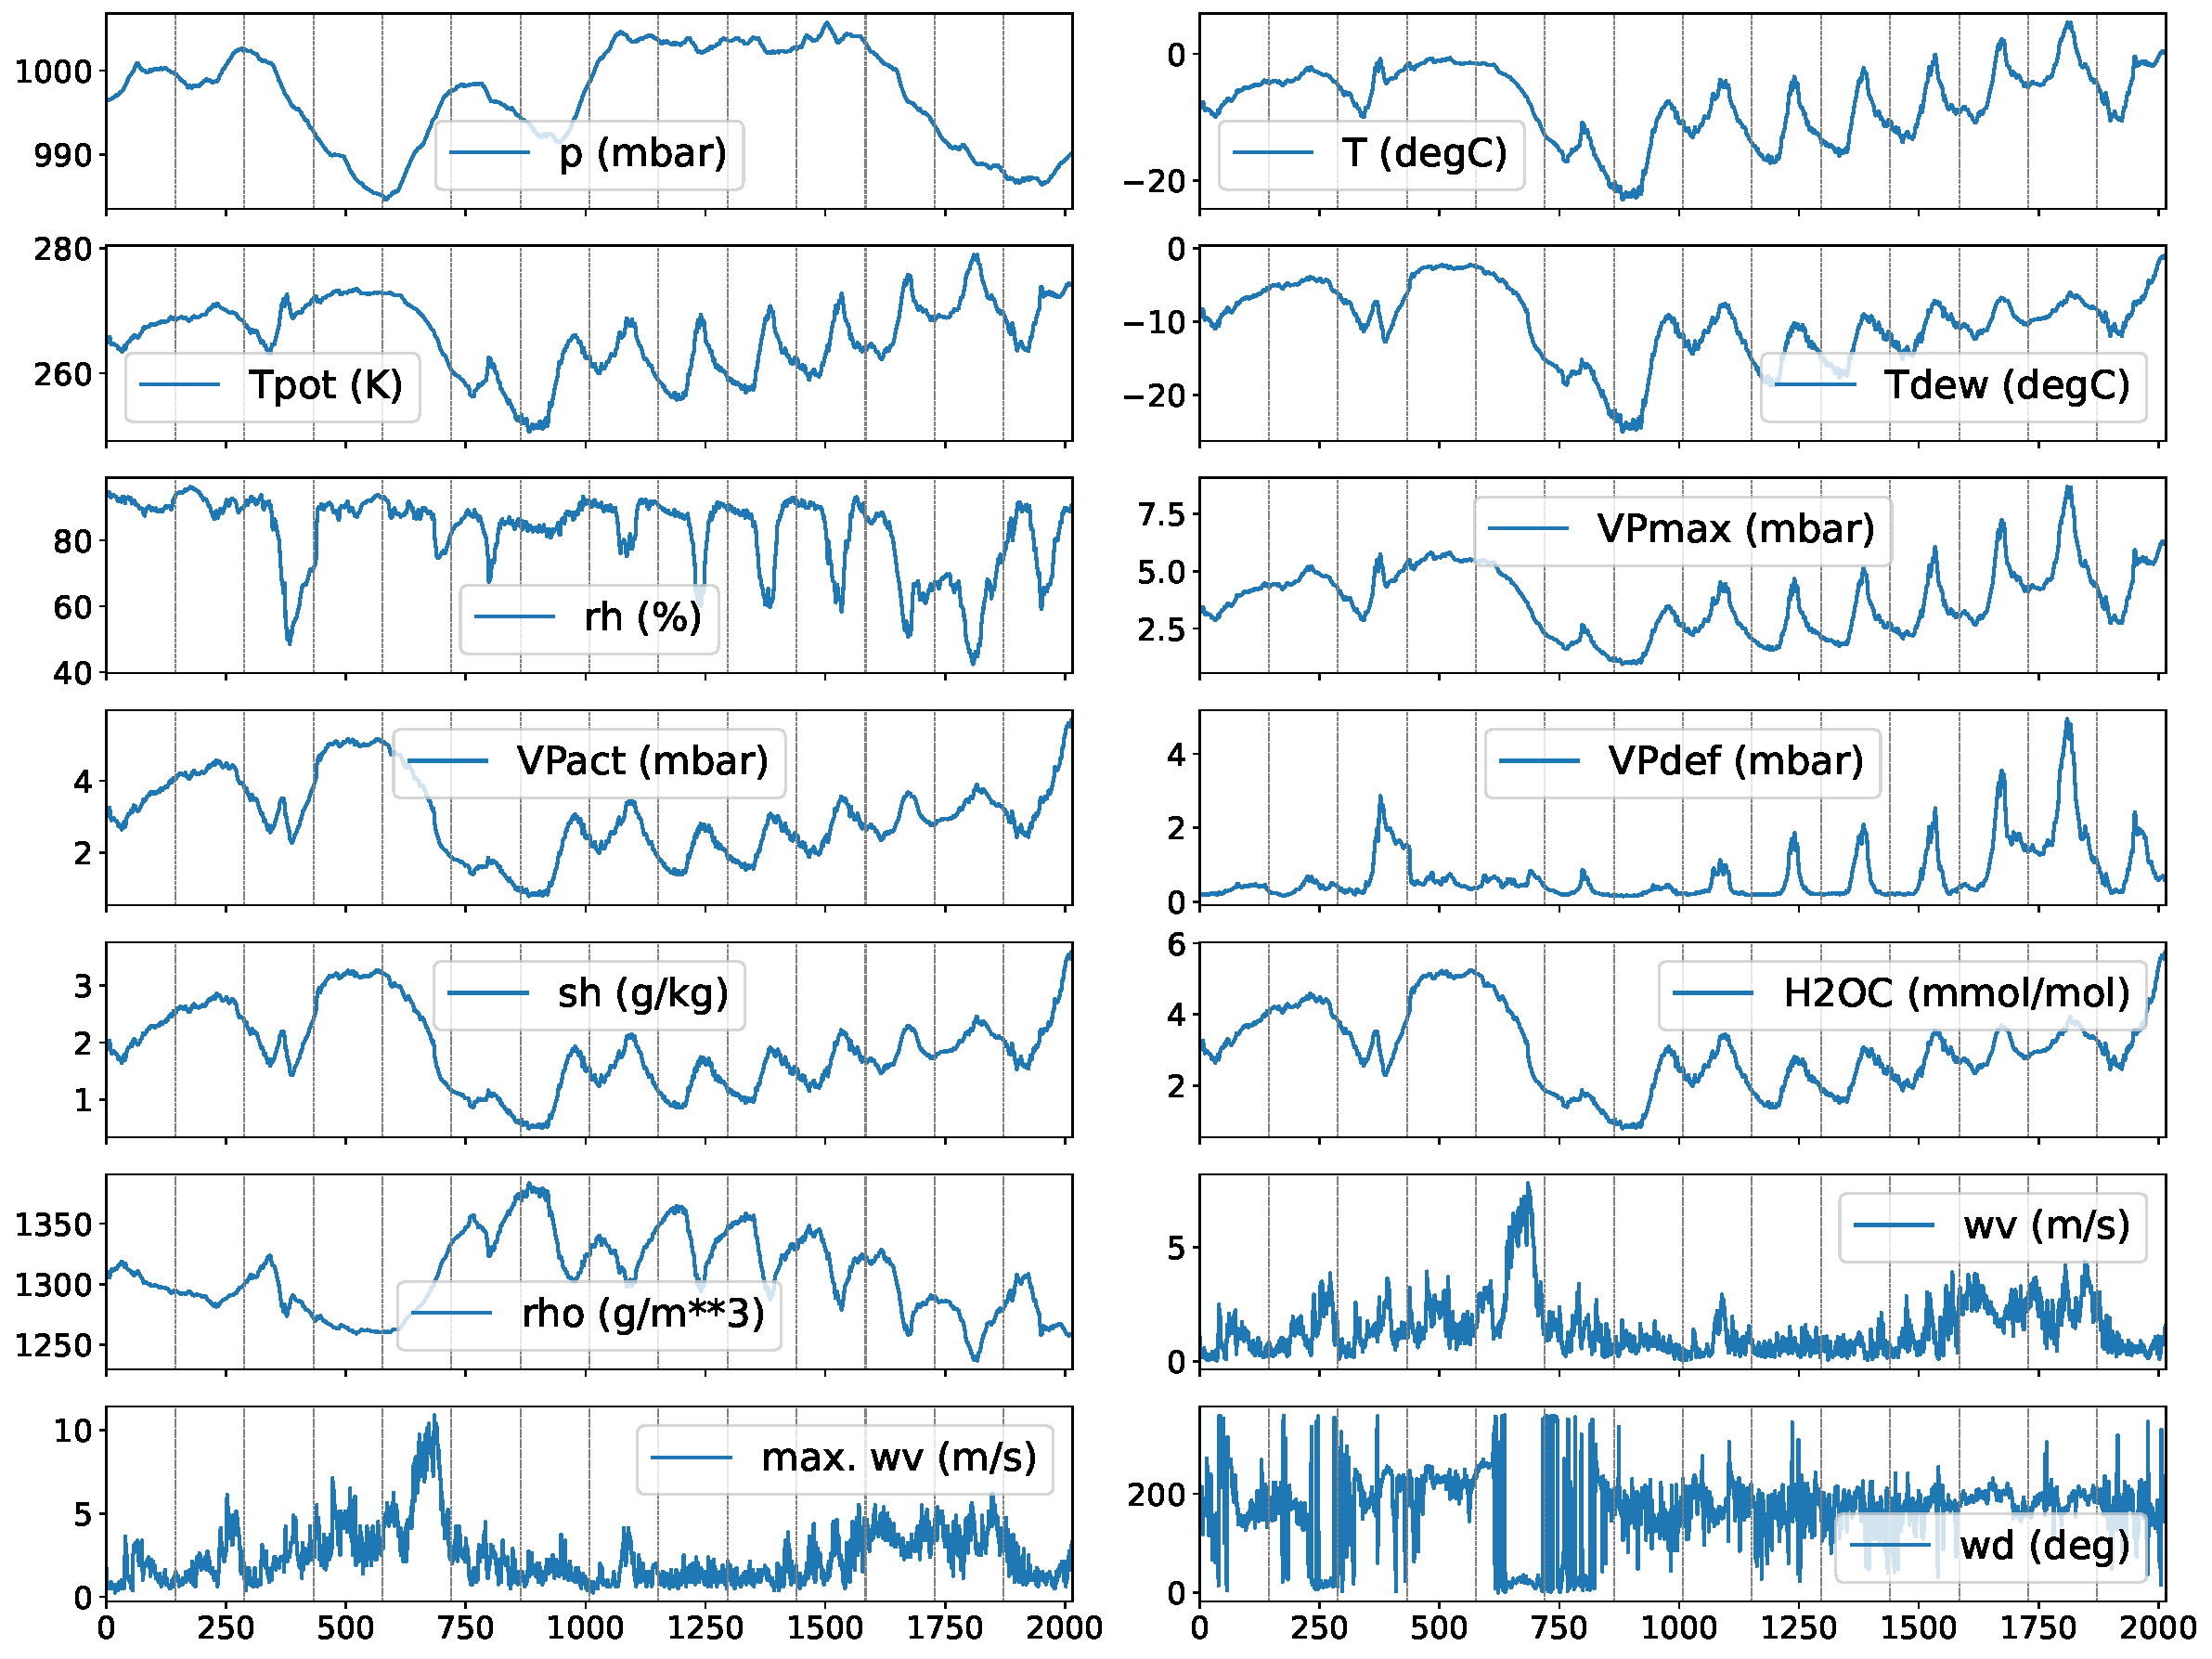
\includegraphics[width=4.675in]{ch_07/fig_07_02} 
	\caption{Timeseries of the Jena Climate Dataset}
	\label{fig:07:02}
\end{figure}

There's some periodicity in the data, such as the daily rise and fall of temperature. You can explore different ranges of data over different timescales by changing the \lstinline{start} and \lstinline{days} parameters in the plotting code.

\begin{nspbox}{Exercise}
\begin{description}
	\item[7-3: Selecting independent features] 
    In the plotted dataset, several measured quantities are so highly correlated that they provide redundant information. Removing irrelevant features can help reduce overfitting, which in turn can improve the model's performance. Additionally, reducing the number of features enhances the explainability of the model by making it easier to understand and interpret.
    
    Analyze the correlations among the quantities to identify redundant features and select a minimal set of representative features, for example, using \emph{correlation matrix analysis}, where where you examine the correlation coefficients between pairs of features to identify those with high correlation (for example, above 0.8 or 0.9) so that you can remove one of the correlated features.
    
    Execute the code of the following sections using all the features and only the minimal set to observe the difference in the performance of the trained model. 
\end{description}
\end{nspbox}

\subsection{Preprocessing the Data}

Now that you've loaded the dataset, your objective is to train a recurrent neural network to predict the temperature at a given time of the day based on the weather information collected during an earlier period---say two days. To do this, you'll need to reformat and normalize the data.

\subsubsection{Reformatting}

First, reshape the data to fit the expected format for training the recurrent neural network to predict temperature, using the code in Listing~\ref{cd:07:reshape}.
\begin{lstlisting}[
    label=cd:07:reshape,
    caption=Reshaping the data for the recurrent neural network
]
n_samples, n_features = data.shape[0], data.shape[1]
(@\codewingding{1}@)past_seq = 2 * daily_samples
(@\codewingding{2}@)lag = 72
(@\codewingding{3}@)temp_idx = 1  # Temperature (Celsius) index.

inputs, targets = [], []
for i in np.random.permutation(range(0, n_samples - past_seq - lag, 
                                     daily_samples)):
    inputs.append(data[i:i + past_seq, :])
    targets.append(data[i + past_seq + lag:i + past_seq + lag + 1, temp_idx])
inputs, targets = np.asarray(inputs), np.asarray(targets)
\end{lstlisting}
This code extracts the total number of samples (\lstinline{n_samples}) and the number of features (\lstinline{n_features}, the 14 different weather data).
Then, it defines the length of the sequences to be fed to the recurrent neural network as inputs \wingding{1} (calculated as the number of days times the number of samples per day); the prediction lag \wingding{2} (how many time steps ahead in time the recurrent neural network should predict temperature---72, providing the temperature at 12:00 of the following day); and the index of the target timeseries to be the temperature in degrees Celsius \wingding{3}.
In the for-cycle, the code fills the inputs with the timeseries and the targets with the values of the temperature at the prediction time. 
Finally, it converts the inputs and targets into NumPy arrays.

Check the \lstinline{inputs} shape using \lstinline{print(inputs.shape)}, which prints \lstinline{(2918, 288, 14)}, and the \lstinline{targets} shape using \lstinline{print(targets.shape)}, which prints
\lstinline{(2918, 1)}. This means that you have 2,918 sequences to train and validate your neural network.

Now, you'll need to determine which sequences to use for training and which to use for validation using Listing~\ref{cd:07:split}.  
\begin{lstlisting}[
    label=cd:07:split,
    caption=Splitting the data into training and validation datasets
]
import deeptrack as dt

sources = dt.sources.Source(inputs=inputs, targets=targets)
train_sources, val_sources = dt.sources.random_split(sources, [0.8, 0.2])
\end{lstlisting}
This code defines the dataset sources and splits them into training and validation datasets in the proportions 80 percent and 20 percent.

\subsubsection{Normalization}

Reviewing Figure~\ref{fig:07:02}, you can see that the data spans a broad range of values with features on considerably different scales, which isn't ideal for neural network training. 
In these conditions, some weights may update faster than others because the feature values influence the magnitude of the gradients used by the backpropagation algorithm. This can lead to slower convergence or even divergence of the learning algorithm. To mitigate these issues, you can rescale all the features to a mean of zero and a standard deviation of one. This step simplifies the network's training. However, be careful not to inadvertently discard crucial information when normalizing your data. 

Listing~\ref{cd:07:stand} normalizes the data by subtracting the mean and dividing by the standard deviation of the training set, using DeepTrack2 pipelines. 
\begin{lstlisting}[
    label=cd:07:stand,
    caption=Normalizing the data
]
import torch

train_mean = np.mean([src["inputs"] for src in train_sources], axis=(0, 1))
train_std = np.std([src["inputs"] for src in train_sources], axis=(0, 1))

inputs_pipeline = (dt.Value(sources.inputs - train_mean) / train_std 
                   >> dt.pytorch.ToTensor(dtype=torch.float))
targets_pipeline = (dt.Value(sources.targets - train_mean[temp_idx]) 
                    / train_std[temp_idx])
\end{lstlisting}
This code calculates the mean and the standard deviation of the training dataset and defines pipelines to normalize the inputs and targets.

\subsubsection{Preparing the Training and Validation Data Loaders}

Finally, prepare the training and validation data loaders with Listing~\ref{cd:07:dataloaders}.
\begin{lstlisting}[
    label=cd:07:dataloaders,
    caption=Defining the data loaders for the training and validation datasets
]
from torch.utils.data import DataLoader

train_dataset = dt.pytorch.Dataset(inputs_pipeline & targets_pipeline, 
                                   inputs=train_sources)
val_dataset = dt.pytorch.Dataset(inputs_pipeline & targets_pipeline, 
                                 inputs=val_sources)

train_loader = DataLoader(train_dataset, batch_size=32, shuffle=True)
val_loader = DataLoader(val_dataset, batch_size=32, shuffle=False)
\end{lstlisting}
This code creates the training and validation datasets and data loaders, which you'll use in the next sections to train and validate the neural networks.

\subsection{Implementing a Common-Sense Benchmark}

You can now introduce a \emph{common-sense benchmark}, which allows you to compare your network's results to some simple standard or ``common sense'' method as a reference. This is good practice in machine learning in general because it provides a baseline to evaluate the performance of your model. Without such a benchmark, it can be difficult to determine if your model is genuinely effective.

For temperature forecasting, a simple benchmark is to assume that the next day's temperature will be equal to the previous day's temperature at the same time.
You can do this with Listing~\ref{cd:07:benchmark}.
\begin{lstlisting}[
    label=cd:07:benchmark,
    caption=Defining a common-sense benchmark
]
temperature = data[:, temp_idx]
(@\codewingding{1}@)benchmark_celsius = np.mean(
    np.abs(
        temperature[daily_samples + lag :: daily_samples] 
        - temperature[lag : -(daily_samples - lag) : daily_samples]
    )
)
(@\codewingding{2}@)benchmark = benchmark_celsius / train_std[temp_idx]
\end{lstlisting}
This code extracts the \lstinline{temperature} timeseries. Then, it calculates the benchmark as the mean absolute error (MAE) between each days' temperatures and the previous days' temperatures at the same time \wingding{1}.
Finally, it normalizes the benchmark by the standard deviation of the training set \wingding{2}.

You can use \lstinline|print(f"Benchmark Celsius: {benchmark_celsius}")| to see the value of the benchmark, which is 2.67$^\circ$C, whereas \lstinline|print(f"Normalized Benchmark: {benchmark}")| shows a normalized benchmark of 0.32.
You'll use the latter value to check whether your trained network outperforma a common-sense benchmark.

You can now implement a recurrent neural network and use it to predict the temperature.
In the following sections, you'll implement different recurrent neural networks and compare them with the common-sense benchmark you just defined.
Before doing that, you need to choose an appropriate device for the computations.

\subsection{Determining the Computation Device}

Training recurrent neural networks is computationally expensive, making it important to select an appropriate device that ensures efficiency and speed. Usually, packages like PyTorch, Lightning, or Deeplay handle this selection automatically. 
However, understanding how to set the device manually can help you optimize the computation, especially when writing models from scratch as you're doing in this chapter.

You can select the device using the \lstinline{get_device()} function in Listing~\ref{cd:07:get_device}.
\begin{lstlisting}[
    label=cd:07:get_device,
    caption=Function to determine the device to be used to perform the computations
]
def get_device():
    """Select device where to perform computations."""
    if torch.cuda.is_available():
        (@\codewingding{1}@)return torch.device("cuda:0")
    elif torch.backends.mps.is_available():
        (@\codewingding{2}@)return torch.device("mps")
    else:
        (@\codewingding{3}@)return torch.device("cpu")
\end{lstlisting}
This function selects a GPU if it's available \wingding{1}\wingding{2}. If not, it selects the CPU \wingding{3}.
The statement \lstinline{"cuda:0"} selects the first GPU if multiple GPUs are available and is equivalent to just \lstinline{"cuda"} for most cases.
The statement \lstinline{"mps"} selects the Apple Silicon GPU device on MacOS, if available.

You can use this function with the code shown in Listing~\ref{cd:07:get_device_call}.
\begin{lstlisting}[
    label=cd:07:get_device_call,
    caption=Selecting the device to be used to perform the computations
]
device = get_device()
\end{lstlisting}
You can now use \lstinline{print(device)} to see which device has been selected, which will depend on your hardware.

\subsection{Predicting with a Simple Recurrent Neural Network}

You can now implement a simple recurrent neural network in PyTorch, as shown in Listing~\ref{cd:07:PT}.
\begin{lstlisting}[
    label=cd:07:PT,
    caption=Defining a recurrent neural network in PyTorch
]
import torch.nn as nn

rnn = nn.RNN(input_size=inputs.shape[2], hidden_size=2, batch_first=True)
fc = nn.Linear(in_features=2, out_features=1)
(@\codewingding{1}@)rnn.to(device); fc.to(device);
\end{lstlisting}
This code defines a simple recurrent neural network with two hidden units (\lstinline{rnn}), which will transform the input timeseries into an output timeseries.
It also defines separately a linear (fully connected) dense layer (\lstinline{fc}), which will take the last element of the output timeseries and use it to estimate the expected temperature.
Finally, it moves the computations to the selected device \wingding{1}.

\subsubsection{Training}

Listing~\ref{cd:07:PTtrain} provides you with a script to train this neural network. This is also a good example of a training loop written in PyTorch from scratch.
\begin{lstlisting}[
    label=cd:07:PTtrain,
    caption=Training the PyTorch recurrent neural network
]
criterion = nn.L1Loss()  # MAE Loss.
(@\codewingding{1}@)parameter_list = list(rnn.parameters()) + list(fc.parameters())
optimizer = torch.optim.Adam(parameter_list, lr=0.001)

epochs = 100
for epoch in range(epochs):
    for inputs, targets in train_loader:
        (@\codewingding{2}@)optimizer.zero_grad()

        (@\codewingding{3}@)inputs, targets = inputs.to(device), targets.to(device)
        (@\codewingding{4}@)rnn_outputs, _ = rnn(inputs)  # RNN layer.
        (@\codewingding{5}@)rnn_outputs = rnn_outputs[:, -1, :]  # Last outputs of timeseries.
        (@\codewingding{6}@)outputs = fc(rnn_outputs)   # Linear layer.
        
        loss = criterion(outputs, targets)
        (@\codewingding{7}@)loss.backward()
        (@\codewingding{8}@)optimizer.step()
    print(f"Epoch {epoch}")
\end{lstlisting}
This code defines the \lstinline{criterion} used to calculate the loss. 
Then it combines the parameters (weights and biases) of the recurrent neural network and the linear layer into one list \wingding{1} which is then passed to the \lstinline{optimizer} to update during training.
Next, it trains the neural network for the set number of epochs.

In each epoch, it iterates over the batches of data provided by \lstinline{train_loader}. 
The loop first resets the gradients of the model parameters to zero to prevent accumulation from previous iterations \wingding{2}. 
Then, it transfers the \lstinline{inputs} and \lstinline{targets} tensors to the device \wingding{3}, feeds the inputs through the recurrent layer \wingding{4}, and selects the last outputs of the timeseries returned by the recurrent layer \wingding{5}. 
It then passes these outputs through the linear layer \wingding{6} to obtain the final output predictions of the next days' temperatures. 
The \lstinline{criterion} computes the \lstinline{loss} between the model's predictions and the actual targets, which is then used to calculate the gradients of the model parameters \wingding{7}. 
Finally, these gradients are used to update the model's weights during the optimization step \wingding{8}.

\subsubsection{Monitoring the Training Loss}

To gain more insights into the training process and ensure that the model is learning effectively, you can update Listing~\ref{cd:07:PTtrain} to print the loss in each epoch, as shown in Listing~\ref{cd:07:PTtrain2}.
Monitoring the training loss helps you detect issues such as overfitting, underfitting, or convergence problems, allowing you to make necessary adjustments to the training parameters or model architecture.
\begin{lstlisting}[
    label=cd:07:PTtrain2,
    caption=Printing the training loss for each epoch (\expand{cd:07:PTtrain})
]
___--snip--___
***train_losses = []***
for epoch in range(epochs):
    ***train_loss = 0.0***
    for inputs, targets in train_loader:
        ___--snip--___
        (@\codewingding{1}@)***train_loss += loss.item()***
    ***train_losses.append(train_loss / len(train_loader))***
    print(f"Epoch {epoch} ***Training Loss: {train_losses[-1]:.4f}***")
\end{lstlisting}
This updated code allows you to observe the training's progress. 
At the beginning of each training epoch, it initializes the \lstinline{train_loss} variable to track the loss accumulated over the epoch.
Then, it adds the loss for each batch to the running total for the epoch \wingding{1}. And 
finally, it saves the loss in the \lstinline{train_losses} NumPy array and prints it.

\subsubsection{Monitoring the Validation Loss}

You can also monitor the evolution of the validation loss during training using Listing~\ref{cd:07:PTtrain3}.
\begin{lstlisting}[
    label=cd:07:PTtrain3,
    caption=Monitoring the evolution of the validation loss
    (\expand{cd:07:PTtrain2})
]
___--snip--___
train_losses***, val_losses*** = []***, []***
for epoch in range(epochs):
    ___--snip--___
    ***val_loss = 0.0
    (@\codewingding{1}@)with torch.no_grad():
        for inputs, targets in val_loader:
            inputs, targets = inputs.to(device), targets.to(device)
            rnn_outputs, _ = rnn(inputs)
            rnn_outputs = rnn_outputs[:, -1, :]
            outputs = fc(rnn_outputs)
            
            loss = criterion(outputs, targets)
            val_loss += loss.item()
    val_losses.append(val_loss / len(val_loader))
    print(f"Epoch {epoch} Validation Loss: {val_losses[-1]:.4f}")***
\end{lstlisting}
This code calculates, saves, and prints the loss for the validation set.
The calculations are similar to those of the training code in Listing~\ref{cd:07:PTtrain}, expect that there is no backpropagation step, so the code is executed without calculating the gradients \wingding{1}.

\subsubsection{Plotting the Training and Validation Losses}

Visualizing the evolution of the training and validation losses can help you identify trends and potential issues during training, such as overfitting or underfitting. To plot the losses during training, you can implement the \lstinline{plot_training()} function shown in Listing~\ref{cd:07:plot_training}.
\begin{lstlisting}[
    label=cd:07:plot_training,
    caption=Function to plot the training and validation losses
]
def plot_training(epochs, train_losses, val_losses, benchmark):
    """Plot the training and validation losses."""
    plt.plot(range(epochs), train_losses, label="Training Loss")
    plt.plot(range(epochs), val_losses, "--", label="Validation Loss")
    plt.plot([0, epochs - 1], [benchmark, benchmark], ":k", label="Benchmark")
    plt.xlabel("Epoch"), plt.xlim([0, epochs - 1])
    plt.ylabel("Loss")
    plt.legend()
    plt.show()
\end{lstlisting}
Then, use it with the command
\begin{lstlisting}
plot_training(epochs, train_losses, val_losses, benchmark)
\end{lstlisting}
which should plot something similar to Figure~\ref{fig:07:03}.

\begin{figure}[H]
	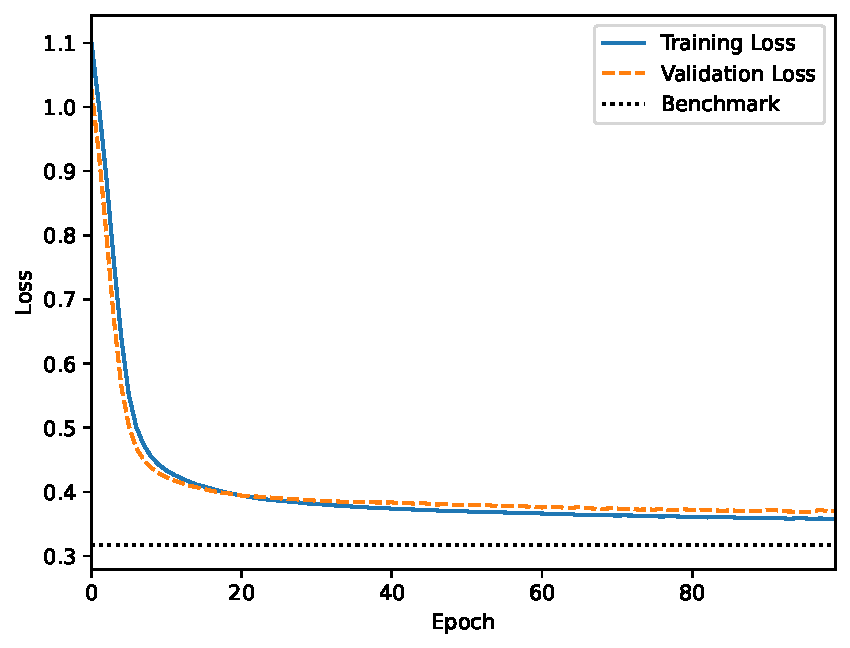
\includegraphics[width=4.675in]{ch_07/fig_07_03} 
	\caption{Training and validation losses for the simple recurrent neural network}
	\label{fig:07:03}
\end{figure}

The training and validation losses both decrease during training, reaching an MAE of about 0.36 for the training loss and 0.38 for the validation loss. Even though these results might appear good, they are worse than the 0.32 MAE obtained with the common-sense benchmark (represented by the dotted line). Therefore, this network has less predictive power than saying that the temperature will be the same as that of the previous day. You'll see how to improve on this in the following sections.

\subsubsection{Implementing the Recurrent Neural Network in Deeplay}

Before proceeding, you can re-implement the previous recurrent neural network in a more compact form using Deeplay, as shown in Listing~\ref{cd:07:DL}.
\begin{lstlisting}[
    label=cd:07:DL,
    caption=Defining a recurrent neural network in Deeplay
]
import deeplay as dl

rnn_dl = dl.RecurrentModel(
    in_features=n_features, 
    hidden_features=[2],
    out_features=1,
    (@\codewingding{1}@)rnn_type="RNN",
)
(@\codewingding{2}@)rnn_simple = dl.Regressor(rnn_dl, optimizer=dl.Adam(lr=0.001)).create()
\end{lstlisting}
Besides the number of input, hidden, and output features, here you can further specify the type of network \wingding{1}, which here is set to \lstinline{"RNN"} (the  default value). 
You can visualize the model architecture using \lstinline{print(model_dl)}.

The code then compiles the neural network as a regression application using the Adam optimizer \wingding{2}. You can print out the details of this compiled application using \lstinline{print(rnn_simple)}.

You can train this recurrent neural network and display the learning curves with the code in Listing~\ref{cd:07:DLtrain}.
\begin{lstlisting}[
    label=cd:07:DLtrain,
    caption=Training the Deeplay recurrent neural network
]
trainer = dl.Trainer(max_epochs=epochs, accelerator="auto")
trainer.fit(rnn_simple, train_loader, val_loader)

train_losses = trainer.history.history["train_loss_epoch"]["value"]
val_losses = trainer.history.history["val_loss_epoch"]["value"][1:]
plot_training(epochs, train_losses, val_losses, benchmark)
\end{lstlisting}
This code creates a trainer that automatically checks the availability of an accelerating device (eliminating the need to use the \lstinline{get_device()} function in Listing~\ref{cd:07:get_device}).
It then proceeds to the training using the \lstinline{fit()} method of the trainer.

The losses calculated during training and validation are automatically logged in the \lstinline{history} field of the trainer, from where you can retrieve them.
The plot of the training and validation losses should be similar to Figure~\ref{fig:07:03}, which you got using the explicit PyTorch implementation in Listings~\ref{cd:07:PTtrain}, \ref{cd:07:PTtrain2}, and \ref{cd:07:PTtrain3}.

\subsection{Stacking Multiple Recurrent Layers}

To enhance the performance of you recurrent neural network, one straightforward strategy is to increase the number of recurrent layers and hidden state features. In fact, stacking multiple recurrent layers can help the network capture more complex patterns and dependencies in the timeseries data.

You can think of \emph{stacked recurrent neural networks} as individual recurrent modules linked together, with the output of one module acting as input to the next. Unlike the output layer where only the final element of the output timeseries is returned, each layer of a stacked recurrent neural networks forwards the entire timeseries it computes to the next layer. This permits each layer to process the entire time-dependent sequence, allowing the network to discover and understand the temporal patterns in the input data.

Similar to the deep convolutional neural networks you encountered in Chapter~\ref{ch:03}, the first layers tend to learn more basic and generic features, while deeper layers can learn task-specific features. In this way, each subsequent layer can build a more sophisticated understanding of the sequential data recognizing complex patterns based on the simpler patterns recognized by the previous layers.

With more parameters to adjust, stacked recurrent neural networks have a greater learning capacity, allowing them to analyze more complex timeseries.  They can remember information over longer sequences, which is beneficial for tasks that require understanding context over long time intervals.

However, stacking recurrent layers has potential downsides.
As the number of layers increases, it becomes more difficult to train the network due to vanishing or exploding gradients, where the gradient becomes too small or too large to propagate useful learning signals through all the layers.
In addition, deeper networks have more parameters and are therefore more prone to overfitting, especially if the training data is limited.

You can implement a stacked recurrent neural network as shown in Listing~\ref{cd:07:DLstacked_rnn}.
\begin{lstlisting}[
    label=cd:07:DLstacked_rnn,
    caption=Defining and training a stacked recurrent neural network
    (\expands{cd:07:DL} and \ref{cd:07:DLtrain})
]
rnn_dl = dl.RecurrentModel(
    in_features=n_features,
    (@\codewingding{1}@)hidden_features=***[16, 16, 16]***,
    out_features=1,
    rnn_type="RNN",
)
***rnn_stacked*** = dl.Regressor(rnn_dl, optimizer=dl.Adam((@\wingding{2}@)lr=***0.0001***)).create()

trainer = dl.Trainer(max_epochs=epochs)
trainer.fit(***rnn_stacked***, train_loader, val_loader)
___--snip--___
\end{lstlisting}
This code updates the recurrent neural network to have three hidden layers, each with 16 features \wingding{1}.
A lower learning rate \wingding{2} helps to smooth out the noise in the loss curve, ensuring more stable convergence during training.

This stacked recurrent neural network has about 1,600 trainable parameters, whereas the simple architecture you used before (Listing~\ref{cd:07:DL}) had only 39.
While thanks to this increased number of trainable parameters the stacked recurrent neural network achieves a better performance than the simple one, it still only reaches an MAE similar to the common-sense benchmark.
This indicates that while stacking layers enhances the model's capacity to learn, further improvement is still necessary. You'll now explore more advanced architectures that achieve better predictive performance.

\subsection{Using Gated Recurrent Units}

Let's now introduce a different type of recurrent neural network known as the \emph{gated recurrent unit} (GRU). 
Figure~\ref{fig:07:04} is a representation of the GRU.

\begin{figure}[H]
	\includegraphics[width=4.675in]{ch_07/fig_07_04} 
	\caption{Gated recurrent unit (GRU)}
	\label{fig:07:04}
\end{figure}

As the name suggests, the GRU is characterized by the use of \emph{gates}, a key feature in modern neural networks inspired by the gating functions found in biological neural systems. 
Gates play a crucial role in regulating the flow of information. They're designed to selectively retain or forget information depending on its relevance for the task at hand. They're typically implemented using activation functions that output values between 0 and 1, acting as switches that can either block or allow information to pass.

GRUs use two types of gates: the update gate and the reset gate. 
The \emph{update gate} helps the model determine how much of the information from previous time steps needs to be passed along. This gate controls the extent to which the previous state influences the current state, balancing between old information and new inputs.

The \emph{reset gate} is responsible for deciding how much of the past information should be forgotten as the network processes new inputs. It allows the GRU to discard information from the past that is deemed unnecessary for the current context or future predictions. A value of the reset gate close to 0 allows the network to nearly forget the previous hidden state, treating the new input as the start of a new sequence. This capability is particularly useful in situations where the sequence contains distinct segments of information that don't benefit from being combined with prior data. In contrast, a value of the reset gate close to 1 retains the previous hidden state, indicating that the new input should be combined with the existing memory to inform the current state.

Since gating introduces additional parameters into the network, you can integrate dropout into the training process to reduce the risk of overfitting. \emph{Dropout} randomly deactivates a subset of neurons during each training iteration, temporarily preventing them from contributing to the data processing. When these neurons are deactivated, other neurons are forced to learn to use also the information previously handled by the deactivated ones. Consequently, various neurons are forced to learn and adapt to the information, ensuring that no single neuron becomes overly specialized to specific traits of the training data. A probability value determines the \emph{dropout rate}, or the likelihood that any given neuron will be turned off at each step. This technique enhances the model's ability to generalize to new, unseen data---for example, to predict tomorrow's temperature. Importantly, dropout is used only during training---all neurons are fully active when the network makes predictions, such as during validation or testing.

Update the network architecture to incorporate a GRU and dropout as shown in Listing~\ref{cd:07:DLstacked_gru}. 
\begin{lstlisting}[
    label=cd:07:DLstacked_gru,
    caption=Defining and training a stacked GRU network
    (\expand{cd:07:DLstacked_rnn})
]
***gru_dl*** = dl.RecurrentModel(
    in_features=n_features,
    hidden_features=***[8, 8, 8]***,
    out_features=1,
    rnn_type=***"GRU"***,
    ***dropout=0.2,***
)
***gru_stacked*** = dl.Regressor(***gru_dl***, optimizer=dl.Adam(lr=***0.001***)).create()
___--snip--___
trainer.fit(***gru_stacked***, train_loader, val_loader)
___--snip--___
\end{lstlisting}
This code sets the network type to GRU and introduces dropout with probability 0.2. The dropout is automatically applied to all the layers except the last one.

Figure~\ref{fig:07:05} shows the resulting learning curves.

\begin{figure}[H]
	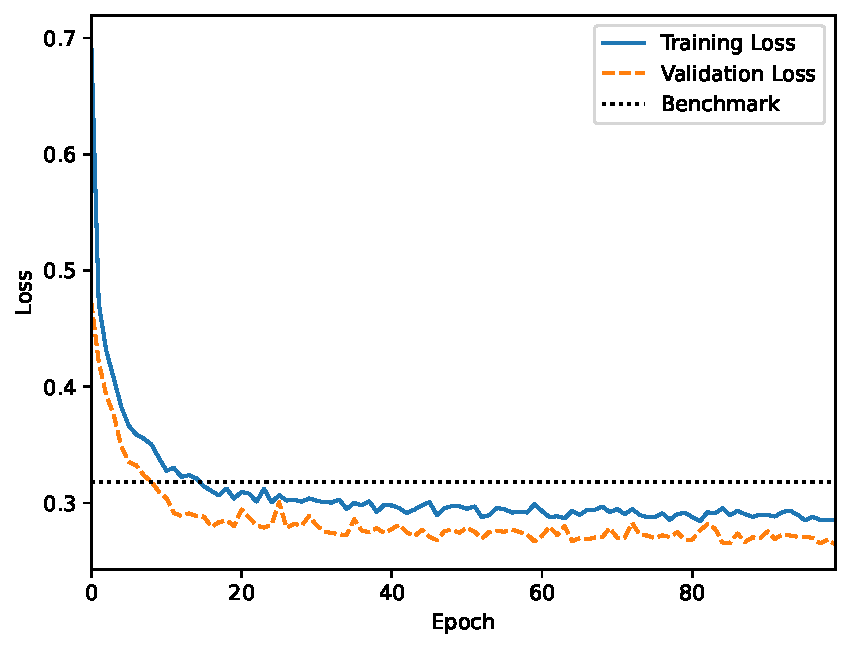
\includegraphics[width=4.675in]{ch_07/fig_07_05} 
	\caption{Training and validation losses for the recurrent neural network implemented with GRUs}
	\label{fig:07:05}
\end{figure}

The learning curves show a noticeable improvement over the simple recurrent neural network shown in Figure~\ref{fig:07:03}, achieving a validation loss of 0.27---substantially lower than the common-sense benchmark.
Interestingly, the validation loss is consistently lower than the training loss throughout the training process thanks to the use of dropout, which randomly deactivates a subset of neurons during each training iteration. During validation, all neurons are active, allowing the model to use the full capacity of its learned features.
In simpler terms, dropout helps the network learn better during training by preventing overfitting, and the model performs even better when all its neurons are used during validation.

\subsection{Using Long Short-Term Memory Networks}

A \emph{long short-term memory} (LSTM) network is an alternative architecture that offers a more sophisticated gating mechanism than GRUs. LSTMs are particularly suited to tasks requiring the capture of long-term dependencies, such as language translation, speech recognition, and time-series forecasting where the influence of earlier data points is significant. Figure~\ref{fig:07:06} shows their structure.

\begin{figure}[H]
	\includegraphics[width=4.675in]{ch_07/fig_07_06} 
	\caption{Long short-term memory (LSTM) unit}
	\label{fig:07:06}
\end{figure}

LSTMs incorporate three gates: the input gate, the forget gate, and the output gate. Together, these gates selectively preserve or eliminate information over different time intervals.
Specifically, the \emph{input gate} evaluates incoming data to identify crucial information to update the state;
the \emph{forget gate} determines how much information from the previous state should be retained or discarded;
and the \emph{output gate} decides the composition of the next hidden state, influencing the network's subsequent outputs.
More gating mechanisms generally results in a higher number of parameters for LSTMs compared to GRUs. This enhances their ability to model complex patterns while also increasing their risk of overfitting.

You can incorporate an LSTM as shown in Listing~\ref{cd:07:DLstacked_lstm}.
\begin{lstlisting}[
    label=cd:07:DLstacked_lstm,
    caption=Defining and training a stacked LSTM network
    (\expand{cd:07:DLstacked_gru})
]
***lstm_dl*** = dl.RecurrentModel(
    ___--snip--___
    rnn_type=***"LSTM"***,
    dropout=***0.3***,
)
***lstm_stacked*** = dl.Regressor(***lstm_dl***, optimizer=dl.Adam(lr=0.001)).create()
___--snip--___
trainer.fit(***lstm_stacked***, train_loader, val_loader)
___--snip--___
\end{lstlisting}
As in the GRU case, this code only requires changing the network type to LSTM. Furthermore, because there're more learnable parameters in the LSTM  than in the GRU, it increases the dropout rate to 0.3. 

Figure~\ref{fig:07:07} shows the resulting learning curves.

\begin{figure}[H]
	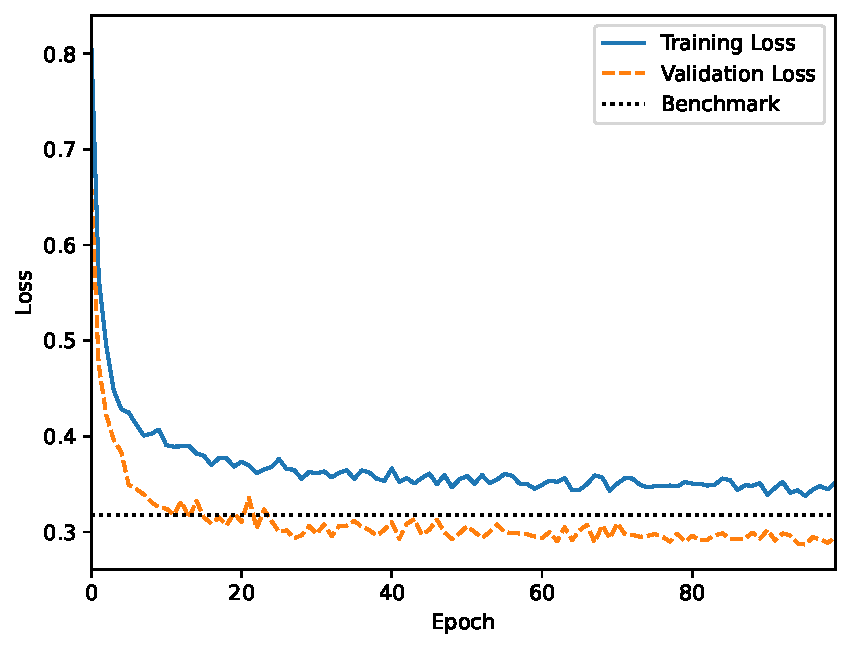
\includegraphics[width=4.675in]{ch_07/fig_07_07} 
	\caption{Training and validation losses for the recurrent neural network implemented with LSTM units}
	\label{fig:07:07}
\end{figure}

The behavior of the learning curves is qualitatively similar to that observed for the GRU in Figure~\ref{fig:07:05}, achieving a similar validation loss of about 0.27 well below the common-sense benchmark.
Note that, while here LSTM units achieve results similar to GRUs, LSTMs are likely to outperform GRUs in more complex tasks where long-term dependencies are crucial, such as in language modeling, speech recognition, or financial timeseries forecasting.

Like in the GRU case, the validation loss remains consistently lower than the training loss because of the use of dropout. In fact, this difference is accentuated by the higher dropout rate of 0.3 used in the LSTM units compared to 0.2 in the GRUs.

\subsection{Code 7-1: Predicting Temperatures using Recurrent Neural Networks}

The \emph{rnn.ipynb} notebook provides the complete code example that uses different kinds of recurrent neural networks to predict the temperature in the Jena Climate Dataset.

\begin{nspbox}{Exercise}
\begin{description}
	\item[7-4: Implementing LSTM with preprocessing]
    Construct a network that combines a stacked LSTM with a preliminary dense network layer for preprocessing, which provides a trainable embedding layer. After training this composite model, evaluate its performance against that of the standalone stacked LSTM.
\end{description}
\end{nspbox}

\section{Project 7A: Translating with a Recurrent Neural Networks}

Recurrent neural networks excel at processing sequences, making them ideal for \emph{natural language processing (NLP)}.
NLP involves the interaction between computers and humans using natural language, with applications ranging from machine translation and sentiment analysis to chatbots. 
Because text sentences are essentially sequences of words, recurrent neural networks can effectively construct \emph{sequence-to-sequence} (\emph{seq2seq}) transformations, enabling the execution of complex linguistic tasks such as translation, summarization, and question-answering.

To understand how this works, consider the task of translation. In a \emph{seq2seq model}, an encoder recurrent neural network reads and processes a source language sentence word by word, capturing the meaning of the entire sentence into in its internal state. This state, often called the \emph{context vector}, is then passed to the decoder. The decoder generates the output sentence. Starting with the context vector from the encoder, it begins generating the sentence in the target language word by word. Each generated word becomes part of the input for the next step in the sequence, along with the updated internal state of the decoder's recurrent neural network. By learning to transform the input sequence (source language sentence) into an output sequence (target language sentence), the model effectively learns to map patterns from one language to another.

For example, given the English sentence ``The cat sits on the mat,'' the encoder processes each word and compresses this information into a context vector. The decoder then takes this vector to produce the Spanish sentence ``El gato se sienta en la alfombra'' one word at a time. This ability to transform sequences enables the model to handle various NLP tasks effectively.

In this project, you'll use recurrent neural networks to implement a seq2seq model to translate sentences from English to Spanish.

\subsection{Preparing the Bilingual Dataset}

To train the seq2seq model, you'll use data from the \emph{ManyThings.org} website at \url{https://www.manythings.org/anki/}. This platform hosts numerous datasets, referred to as ``Anki decks'', which consist of flashcards with bilingual sentence pairs across various language combinations. Each dataset is downloadable in a simple text format, typically as \emph{.txt} files with the naming convention \emph{language\_1-language\_2.txt}. This file is know as a \emph{corpus file} and contains thousands of sentence pairs, where each pair consists of a sentence in one language and its translation in another. This structure makes them ideally suited for training translation models.

You'll use the \emph{eng-spa.txt} file with English-to-Spanish translations.
Some excerpts from this file are:
\begin{lstlisting}
Go.	Ve.	CC-BY 2.0 (France) Attribution: ...
Go.	Vete.	CC-BY 2.0 (France) Attribution: ...
Go.	Vaya.	CC-BY 2.0 (France) Attribution: ...
Go.	Váyase.	CC-BY 2.0 (France) Attribution: ...
Hi.	Hola.	CC-BY 2.0 (France) Attribution: ...
___--snip--___
Cheer up!	¡Anímate!	CC-BY 2.0 (France) Attribution: ...
Cheer up!	Anímate.	CC-BY 2.0 (France) Attribution: ...
Cheer up.	Venga.	CC-BY 2.0 (France) Attribution: ...
___--snip--___
\end{lstlisting}
Each line consists of a sentence in English followed by its Spanish translation with some metadata at the end, separated by tab characters.

Before using the data for training, some preprocessing is necessary. Chapter~\ref{ch:08} will explain the different preprocessing steps common in NLP tasks in more detail. For now, you need to tokenize and filter the sentences to remove the metadata and ensure the text is in a clean, standardized format. 

%\subsubsection{Tokenizing the Sentences}

First, you'll need to break down sentences into words, a process called \emph{tokenization}. You'll do this through the \lstinline{tokenize()} function provided in Listing~\ref{cd:07:A:tokenize}. This function also handles contractions, standardizes quotation marks, and filters out unwanted tokens.
\begin{lstlisting}[
    label=cd:07:A:tokenize,
    caption=Function to tokenize and standardize text
]
import contractions, re
from torchtext.data.utils import get_tokenizer

tokenizer_eng = get_tokenizer("spacy", language="en_core_web_sm")
tokenizer_spa = get_tokenizer("spacy", language="es_core_news_sm")

def tokenize(text, lang):
    """Standardize, tokenize and filter text."""
    (@\codewingding{1}@)text = (text.replace("’", "'").replace("‘", "'").replace("´", "'")
            .replace("“", '"').replace("”", '"').replace("´´", '"'))
    tokens = ((@\wingding{2}@)tokenizer_eng(contractions.fix(text)) if lang == "eng"
              else (@\wingding{3}@)tokenizer_spa(text))  # lang == "spa"
    (@\codewingding{4}@)filtered_tokens = [token for token in tokens if re.match(
        r"""
        ^[a-zA-Z0-9áéíóúüñÁÉÍÓÚÜÑ.,!?¡¿]+  # 1+ allowed characters.
        (-[a-zA-Z0-9áéíóúüñÁÉÍÓÚÜÑ.,!?¡¿]+)*  # Optional hyphen plus chars.
        (_[a-zA-Z0-9áéíóúüñÁÉÍÓÚÜÑ.,!?¡¿]+)*  # Optional underscore plus chars.
        $  # End of the string.
        """, token, re.VERBOSE)]
    return filtered_tokens
\end{lstlisting}
This code initializes English (\lstinline{tokenizer_eng}) and Spanish (\lstinline{tokenizer_spa}) tokenizers using spaCy models. Loading spaCy models can be time-consuming because it involves loading large model files into memory and initializing various components. To minimizes the initialization overhead, which would significantly slow down the execution of the code, the code runs this initialization outside the \lstinline{tokenize} function.

The \lstinline{tokenize()} function first standardizes quotation marks and apostrophes to ensure uniformity across the text \wingding{1}.
Then, if the selected language is English, it scans the input text for any known contractions and replaces them with their expanded forms before tokenizing it with the English tokenizer \wingding{2}.
If the selected language is Spanish, it just tokenizes the text with the Spanish tokenizer \wingding{3}.
Finally, the function filters out tokens that don't match a predefined pattern of allowed characters and symbols \wingding{4}.  The pattern includes letters, numbers, accented characters, punctuation marks, and certain special characters. This filtering ensures that only relevant tokens are retained for further processing, excluding any unwanted or malformed tokens that do not contribute to the language processing tasks.

Now you need the \lstinline{corpus_iterator()} function in Listing~\ref{cd:07:A:corpus_iterator} to apply this tokenization to all the sentences contained in the data file.
\begin{lstlisting}[
    label=cd:07:A:corpus_iterator,
    caption=Function to read and tokenize sentences by iterating through a corpus file
]
def corpus_iterator(filename, lang, lang_position):
    """Read and tokenize texts by iterating through a corpus file."""
    with open(filename, "r", encoding="utf-8") as file:
        for line in file:
            sentences = line.strip().split("\t")
            sentence = sentences[lang_position]
            yield tokenize(sentence, lang)
\end{lstlisting}
This function starts by opening the specified file in read mode with UTF-8 encoding to ensure compatibility with different languages and special characters. 
It reads the file line by line, where each line contains a sentence in the source language and its translation in the target language, separated by a tab character. The function strips any extraneous whitespace from the line and splits it into components based on the tab character. 
It then selects either the first (English) or second (Spanish) element (identified by \lstinline{lang_position}) of the split line as the sentence to be tokenized. Finally, it tokenizes the selected text using the \lstinline{tokenize()} function and yields the tokenized sentence for further processing.

\subsection{Building the Vocabularies}

In translation tasks, constructing comprehensive vocabularies is essential. To build a high-quality vocabulary that is extensive and representative of the language used in the text corpus, you need to process a given text corpus to identify and catalog every unique word. 
For this task, you'll use the function \lstinline{build_vocab()} in Listing~\ref{cd:07:A:build_vocab}.
\begin{lstlisting}[
    label=cd:07:A:build_vocab,
    caption=Function to build a vocabulary from a corpus file
]
from torchtext.vocab import build_vocab_from_iterator

def build_vocab(filename, lang, lang_position, specials="<unk>", min_freq=5):
    """Build vocabulary."""
    vocab = build_vocab_from_iterator(
        corpus_iterator(filename, lang, lang_position),
        min_freq=min_freq,
        specials=specials,
    )
    (@\codewingding{1}@)vocab.set_default_index(vocab[specials[-1]])
    return vocab
\end{lstlisting}
This function uses the \lstinline{build_vocab_from_iterator()} TorchText function to construct the vocabulary using the iterator returned by the \lstinline{corpus_iterator()} function. The \lstinline{min_freq} parameter sets the minimum frequency a word must have to be included in the vocabulary and the \lstinline{specials} parameter sets the special tokens that need to be included in the vocabulary. These special tokens, such as \lstinline{<unk>} (unknown), \lstinline{<pad>} (padding), \lstinline{<bos>} (beginning of sentence), and \lstinline{<eos>} (end of sentence), are crucial for handling common NLP tasks like padding sequences to the same length or marking sentence boundaries. 
Finally, the default index for the vocabulary is set to the index of the last special token \wingding{1}. If no special tokens are indicated, this will be set by default to the string \lstinline{<unk>}.

Use this function to create the vocabularies for the input and output languages as shown in Listing~\ref{cd:07:A:build_vocab2}.
\begin{lstlisting}[
    label=cd:07:A:build_vocab2,
    caption=Building the vocabularies
]
in_lang, out_lang, filename = "eng", "spa", "eng-spa.txt"
special_tokens = ["<pad>", "<sos>", "<eos>", "<unk>"]

in_vocab = build_vocab(filename, in_lang, lang_position=0, 
                       specials=special_tokens)
out_vocab = build_vocab(filename, out_lang, lang_position=1, 
                        specials=special_tokens)
\end{lstlisting}
This code defines the input language (\lstinline{in_lang}) and the output language (\lstinline{out_lang}) as well as the file name containing the list of translated sentences.
It then defines the list of special tokens that need to be included in the vocabularies: \lstinline{"<pad>"} for padding; \lstinline{"<sos>"} for start of a sequence; \lstinline{"<eos>"} for end of a sequence; and \lstinline{"<unk>"} for unknown words. 
Finally, it builds the vocabularies for the input language (\lstinline{in_vocab}) and for the target language (\lstinline{out_lang}).

\subsection{Preprocessing the Data}

To use a corpus for training a network for translation tasks, sentences must be tokenized, validated against a vocabulary, padded to ensure that all sequences are of a consistent length, and transformed into a format suitable for machine learning models. 

You'll need the \lstinline{all_words_in_vocab()} function in Listing~\ref{cd:07:A:all_words_in_vocab} to check whether all words in a sentence are present in a vocabulary.
\begin{lstlisting}[
    label=cd:07:A:all_words_in_vocab,
    caption=Function to check if all words in a sentence are present in a vocabulary
]
def all_words_in_vocab(sentence, vocab):
    """Check whether all words in a sentence are present in a vocabulary"""
    return all(word in vocab for word in sentence)
\end{lstlisting}
%This function checks whether all words in a given sentence are present in a specified vocabulary, ensuring that the data fed into a model only contains known words. 

Then, you'll need the \lstinline{pad()} function in Listing~\ref{cd:07:A:pad} to pad a sequence of tokens to a predefined length.
\begin{lstlisting}[
    label=cd:07:A:pad,
    caption=Function to pad a sequence of tokens
]
def pad(tokens, max_length=10):
    """Pad sequence of tokens."""
    padding_length = max_length - len(tokens)
    return ["<sos>"] + tokens + ["<eos>"] + ["<pad>"] * padding_length
\end{lstlisting}
This function takes a sequence of words, adds the special tokens for the start of sentence (\lstinline{"<sos>"}) and for the end of sentence (\lstinline{"<eos>"}), and pads it to a designated maximum length using a padding token (\lstinline{"<pad>"}).

Finally, you'll need the \lstinline{process()} function in Listing~\ref{cd:07:A:process} to process the entire language corpus.
\begin{lstlisting}[
    label=cd:07:A:process,
    caption=Function to process the language corpus
]
import numpy as np

def process(file, in_lang, out_lang, in_vocab, out_vocab, max_length=10):
    """Process language corpus."""
    in_sequences, out_sequences = [], []
    for line in file:
        (@\codewingding{1}@)sentences = line.strip().split("\t")
        in_tokens = tokenize(sentences[0], in_lang)
        out_tokens = tokenize(sentences[1], out_lang)

        if (all_words_in_vocab(in_tokens, in_vocab)
            and len(in_tokens) <= max_length
            and all_words_in_vocab(out_tokens, out_vocab)
            and len(out_tokens) <= max_length):
            
            padded_in_tokens = pad(in_tokens)
            in_sequence = in_vocab(padded_in_tokens)
            in_sequences.append(in_sequence)
            
            padded_out_tokens = pad(out_tokens)
            out_sequence = out_vocab(padded_out_tokens)
            out_sequences.append(out_sequence)

    return np.array(in_sequences), np.array(out_sequences)
\end{lstlisting}
This function reads each line and splits it into input and target text sequences based on a tab delimiter \wingding{1}. Then, it tokenizes them (\lstinline{in_tokens} and \lstinline{out_tokens}). 
If \lstinline{in_tokens} and \lstinline{out_tokens} meet a set of criteria (all words are in the respective vocabularies and don't exceed the maximum length), it pads them, transforms them into numerical data according to the vocabulary index, and appends them to the \lstinline{in_sequences} and \lstinline{out_sequences} lists. The output lists are finally converted into NumPy arrays and returned.

You can now use the \lstinline{process()} function to preprocess the text corpus and the preprocessed data as a source to build the data loaders, as shown in Listing~\ref{cd:07:A:dataloaders}.
\begin{lstlisting}[
    label=cd:07:A:dataloaders,
    caption=Building the datasets and data loaders
]
import deeptrack as dt
import torch
from torch.utils.data import DataLoader

with open(filename, "r", encoding="utf-8") as file:
    in_sequences, out_sequences = \
        process(file, in_lang, out_lang, in_vocab, out_vocab)

sources = dt.sources.Source(inputs=in_sequences, targets=out_sequences)
train_sources, test_sources = dt.sources.random_split(sources, [0.85, 0.15])

inputs_pip = dt.Value(sources.inputs) >> dt.pytorch.ToTensor(dtype=torch.int)
outputs_pip = dt.Value(sources.targets) >> dt.pytorch.ToTensor(dtype=torch.int)

train_dataset = \
    dt.pytorch.Dataset(inputs_pip & outputs_pip, inputs=train_sources)
test_dataset = \
    dt.pytorch.Dataset(inputs_pip & outputs_pip, inputs=test_sources)

train_loader = DataLoader(train_dataset, batch_size=256, shuffle=True)
test_loader = DataLoader(test_dataset, batch_size=256, shuffle=False)
\end{lstlisting}
This code begins by processing the dataset with the \lstinline{process()} function. It creates a source to house both the inputs and targets, providing a structured way to handle paired data necessary for supervised learning tasks. Then, the code splits the \lstinline{sources} object into training and test sets according to the proportions 85 percent and 15 percent, respectively. Next, it creates DeepTrack2 pipelines for both inputs (\lstinline{inputs_pip}) and targets (\lstinline{outputs_pip}) to transform data into PyTorch tensors. To manage data for training, the \lstinline{train_dataset} and \lstinline{test_dataset} objects are instantiated, associating inputs and targets with their respective sources. Finally, the \lstinline{train_loader} and \lstinline{test_loader} data loaders are created to handle data batching.

\subsection{The Sequence-to-Sequence Architecture}

A typical seq2seq model consists of two main components: an encoder and a decoder. 
%The roles and functionalities of encoders and decoders are distinct yet complementary, each serving a specific purpose. 
The encoder focuses on reading and understanding the input sequence, such as a sentence in English, compressing it into a rich context---a summary that captures the meaning of the entire input sequence. This context is like a mental snapshot of what the input sequence represents.
The decoder then takes this context and transforms this context into a meaningful output sequence, such as translating the summary into a Spanish sentence. The decoder generates the output one word at a time, using the context provided by the encoder to ensure that the translation is accurate and coherent.

\subsubsection{Implementing the Encoder}

The encoder reads the input sequence and converts each word into \emph{embeddings}, which are dense vector representations of the words. These embeddings capture the semantic meaning of the words in a way that the neural network can process. Each word's embedding is then fed into a recurrent neural network. With each word processed, the recurrent neural network updates its internal state. After processing the last word, the final state of the recurrent neural network represents the entire sentence---a compact representation of the meaning and context of the input sequence.
Listing~\ref{cd:07:A:encoder} shows the \lstinline{Seq2SeqEncoder} class.
\begin{lstlisting}[
    label=cd:07:A:encoder,
    caption=Class implementing the encoder network
]
import deeplay as dl

class Seq2SeqEncoder(dl.DeeplayModule):
    """Sequence-to-sequence encoder."""

    def __init__(self, vocab_size, in_features=300, hidden_features=128,
                 hidden_layers=1, dropout=0.0, bidirectional=True):
        """Initialize sequence-to-sequence encoder."""
        super().__init__()

        self.hidden_features = hidden_features
        self.hidden_layers = hidden_layers
        self.bidirectional = bidirectional
        (@\codewingding{1}@)self.embedding = dl.Layer(torch.nn.Embedding, vocab_size, in_features)
        (@\codewingding{2}@)self.rnn = dl.Layer(torch.nn.GRU, input_size=in_features, \
            hidden_size=hidden_features, num_layers=hidden_layers, \
            dropout=(0 if hidden_layers == 1 else dropout), \
            bidirectional=bidirectional, batch_first=True)

    def forward(self, in_sequences, hidden=None):
        """Perform forward pass."""
        in_sequences = self.embedding(in_sequences)
        encoder_outputs, hidden = self.rnn(in_sequences, hidden)
        (@\codewingding{3}@)if self.bidirectional:
            encoder_outputs = (encoder_outputs[:, :, :self.hidden_features]
                               + encoder_outputs[:, :, self.hidden_features:])
            hidden = hidden[:self.hidden_layers]
        return encoder_outputs, hidden
\end{lstlisting}
The encoder has two main module components: the embedding layer \wingding{1} and the recurrent neural network layer \wingding{2}. 
The embedding layer converts token indices into dense vectors of a fixed size. It is initialized with the vocabulary size and the number of input features. The recurrent neural network layer is instantiated with the type of recurrent neural network, number of hidden layers, bidirectionality, and dropout. This layer processes the sequence of embedded tokens and produces outputs and a hidden state.

The \lstinline{forward()} method defines how the input sequence is transformed as it passes through the network layers. It takes an input sequence and an optional hidden state. The input sequence first passes through the embedding layer. The recurrent neural network layer then processes the embedded sequence, returning the output sequence and a new hidden state. If the recurrent neural network is bidirectional \wingding{3}, the outputs from both directions are summed to combine the forward and backward contextual information, and the hidden state from the backward pass is discarded, retaining only the hidden state from the forward pass.

\subsubsection{Implementing the Decoder}

The decoder's role is to generate an output sequence from the encoded data. It translates the context or hidden states provided by the encoder into a new sequence, translating the input sentence into the target language. 
Listing~\ref{cd:07:A:decoder} shows the \lstinline{Seq2SeqDecoder} class that implements the decoder network by taking the context vector from the encoder and generating the target sequence step by step.
\begin{lstlisting}[
    label=cd:07:A:decoder,
    caption=Class implementing the decoder network
]
class Seq2SeqDecoder(dl.DeeplayModule):
    """Sequence-to-sequence decoder."""

    def __init__(self, vocab_size, in_features=300, hidden_features=128, 
                 hidden_layers=1, dropout=0.0):
        """Initialize sequence-to-sequence decoder."""
        super().__init__()

        self.embedding = dl.Layer(torch.nn.Embedding, vocab_size, in_features)
        self.rnn = dl.Layer(torch.nn.GRU, input_size=in_features, \
            hidden_size=hidden_features, num_layers=hidden_layers, \
            bidirectional=False, batch_first=True, \
            dropout=(0 if hidden_layers == 1 else dropout))
        self.dense = dl.Layer(torch.nn.Linear, hidden_features, vocab_size)
        self.softmax = dl.Layer(torch.nn.Softmax, dim=-1)
        self.relu = dl.Layer(torch.nn.ReLU)

    def forward(self, x, hidden):
        """Perform forward pass."""
        x = self.embedding(x)
        (@\codewingding{1}@)x = self.relu(x)
        (@\codewingding{2}@)output, hidden = self.rnn(x, hidden)
        (@\codewingding{3}@)output = self.dense(output)
        (@\codewingding{4}@)output = self.softmax(output)
        return output, hidden
\end{lstlisting}
The decoder has a similar structure as the encoder. However, it's typically unidirectional because it generates the output sequence in the forward direction, building on previously generated tokens. 

The \lstinline{forward()} method shows that the decoder is more complex than the encoder because it needs to generate coherent and contextually appropriate outputs.
After the embedding, tokens are passed through a ReLU activation function, which introduces non-linearity helping the network learn more complex patterns \wingding{1}. Then,the recurrent neural network processes the activated embeddings along with the initial hidden state to produce output for each time step and a new hidden state \wingding{2}. Each output from the recurrent neural network is transformed by the dense layer \wingding{3} and then converted into a probability distribution across the vocabulary by the softmax function \wingding{4}. The softmax probabilities (which can be interpreted as the next token predictions) and the new hidden state are returned for use in subsequent time steps.

\subsubsection{Combining the Encoder and the Decoder}

Now that you've implemented both the encoder and the decoder, you can combine them into the full seq2seq model to translate text sequences from one language to another, as shown in Listing~\ref{cd:07:A:seq2seq}.
\begin{lstlisting}[
    label=cd:07:A:seq2seq,
    caption=Class implementing the full seq2seq model
]
class Seq2SeqModel(dl.DeeplayModule):
    """Sequence-to-sequence model."""

    def __init__(self, in_vocab_size=None, out_vocab_size=None,
                 teacher_prob=1.0, embedding_dim=300, hidden_features=128,
                 hidden_layers=1, dropout=0.0, bidirectional=True):
        """Initialize the sequence-to-sequence model."""
        super().__init__()
        
        self.out_vocab_size = out_vocab_size
        self.teacher_prob = teacher_prob
        self.encoder = Seq2SeqEncoder(in_vocab_size, embedding_dim, \
            hidden_features, hidden_layers, dropout, bidirectional)
        self.decoder = Seq2SeqDecoder(out_vocab_size, embedding_dim, \
            hidden_features, hidden_layers, dropout)

    def forward(self, batch):
        """Perform forward pass."""
        in_sequences, out_sequences = batch
        
        (@\codewingding{1}@)_, encoder_hidden = self.encoder(in_sequences)
        (@\codewingding{2}@)decoder_hidden = encoder_hidden
        (@\codewingding{3}@)decoder_outputs = torch.zeros(
            (out_sequences.size(0), out_sequences.size(1), self.out_vocab_size)
        ).to(next(self.encoder.parameters()).device)        

        (@\codewingding{4}@)for t in range(in_sequences.size(1)):
            if t == 0 or np.random.rand() < self.teacher_prob:
                (@\codewingding{5}@)decoder_input = out_sequences[:, t].unsqueeze(-1)
            else:
                (@\codewingding{6}@)decoder_input = top1.squeeze(-1).detach()

            decoder_input = \
                decoder_input.to(next(self.decoder.parameters()).device)
            decoder_output, decoder_hidden = \
                self.decoder(decoder_input, decoder_hidden)
            _, top1 = decoder_output.topk(1)
            decoder_outputs[:, t, :] = decoder_output.squeeze(1)
        return decoder_outputs

    def evaluate(self, in_sequences):
        """Evaluate model."""
        with torch.no_grad():
            _, encoder_hidden = self.encoder(in_sequences)
        decoder_hidden = encoder_hidden
        out_sequences = torch.zeros(
            in_sequences.shape,
        ).to(next(self.encoder.parameters()).device)
        
        for t in range(in_sequences.size(1)):
            if t == 0:
                decoder_input = \
                    torch.full(size=(in_sequences.size(0), 1), fill_value=1,
                               device=next(self.encoder.parameters()).device)
            else:
                decoder_input = top1.squeeze(-1).detach()

            decoder_input = \ 
                decoder_input.to(next(self.decoder.parameters()).device)
            with torch.no_grad():
                decoder_output, decoder_hidden = \
                    self.decoder(decoder_input, decoder_hidden)
            _, top1 = decoder_output.topk(1)
            out_sequences[:, t] = top1.squeeze()
        return out_sequences
\end{lstlisting}
This class combines the encoder and the decoder.
In the \lstinline{forward()} method, the input sequence is first passed through the encoder, which generates a set of outputs and a hidden state that captures the contextual information of the input sequence \wingding{1}.
Then, the decoder hidden state is set to be equal to the encoder hidden state \wingding{2}. Its output is initialized to a tensor of zeros and moved to the same device as the encoder's parameters \wingding{3}.
As a result, the decoder uses the encoder’s hidden state as its initial state and starts generating the output sequence. 

The decoder output is constructed step-by-step \wingding{4}. Each step's output depends on the previous steps' outputs, making the process inherently sequential and dependent on prior results. The model uses \emph{teacher forcing} as a training strategy, where the actual target token (the correct translation from the ground truth) is used as the next input to the decoder with probability \lstinline{teacher_prob} \wingding{4}, while otherwise the model’s prediction from the previous time step is used \wingding{5}.
Setting \lstinline{teacher_prob} to different levels has various effects: a high probability (closer to 1) helps the model learn more quickly and accurately when the correct sequences are provided but may cause the model to struggle during inference without the ground truth; a low probability (closer to 0) makes the model more robust to errors and improves performance during inference, though it may slow down the training process and make convergence less stable. Finding the right balance is key to effective training and often involves some experimentation.
When training recurrent neural networks, this strategy speeds up training and often leads to more stable convergence. However, it can also lead to the model becoming overly reliant on the ground truth during training and not learning to recover from its own mistakes---a phenomenon called \emph{exposure bias}.

To evaluate the model on unseen data, the class has an \lstinline{evaluate()} method that uses a similar approach to the \lstinline{forward()} method but without teacher forcing, because during evaluation, you simulate the inference process while the model doesn't have access to the ground truth for the next token, and with all operations performed with the gradient computations disabled, which reduces memory usage and speeds up the evaluation process.

\subsubsection{Defining the Loss Function}

For the loss function, you'll use the \emph{negative log-likelihood loss}, which measures the performance of a classification model whose output is a probability value between 0 and 1.
However, padding tokens should be ignored for the loss function calculation so that the model's training process focuses solely on the meaningful part of the sequence.
The \lstinline{maskedNLL()} function in Listing~\ref{cd:07:A:loss} is an efficient way to calculate a masked version of the negative log-likelihood for batched data. 
\begin{lstlisting}[
    label=cd:07:A:loss,
    caption= Function to calculate the masked negative log-likelihood loss
]
def maskedNLL(in_sequences, out_sequences, PADtoken=0):
    """Calculate the negative log-likelihood loss."""
    mask = out_sequences != PADtoken
    NLL = - torch.log(
        torch.gather(in_sequences.view(-1, in_sequences.shape[-1]), 
                     1, out_sequences.view(-1, 1))
    )
    loss = NLL.masked_select(mask.view(-1, 1)).mean()
    return loss
\end{lstlisting}
This function first creates \lstinline{mask}, a boolean tensor that identifies where the target tensor’s elements are different from the pad token. 
A crucial step for efficiency is using the \lstinline{torch.gather()} function to select the specific entries in the input tensor, which contains probability outputs for each class for each predicted word corresponding to the actual class labels in the target.

\subsubsection{Implementing the Sequence-to-Sequence Application}

Finally, you're ready to define a class \lstinline{Seq2Seq()} by extending the \lstinline{Application} class of Deeplay, as showcased in Listing~\ref{cd:07:A:applic}.
\begin{lstlisting}[
    label=cd:07:A:applic,
    caption=Class implementing the application to train the seq2seq model
]
class Seq2Seq(dl.Application):
    """Application for the sequence-to-sequence model."""

    def __init__(self, in_vocab, out_vocab, teacher_prob=1.0):
        """Initialize the application."""
        super().__init__(loss=maskedNLL, optimizer=dl.Adam(lr=1e-3))
        (@\codewingding{1}@)self.model = Seq2SeqModel(in_vocab_size=len(in_vocab), \
            out_vocab_size=len(out_vocab), teacher_prob=teacher_prob)

    def train_preprocess(self, batch):
        """Adjust the target sequence by shifting it one position backward."""
        in_sequences, out_sequences = batch
        shifted_out_sequences = \
            torch.cat((out_sequences[:, 1:], out_sequences[:, -1:]), dim=1)
        return (in_sequences, out_sequences), shifted_out_sequences
    
    def forward(self, batch):
        """Perform forward pass."""
        return self.model(batch)
\end{lstlisting}
This class creates a default model from the \lstinline{Seq2SeqModel} class in Listing~\ref{cd:07:A:seq2seq} \wingding{1}, which uses the \lstinline{maskedNLL()} function defined in Listing~\ref{cd:07:A:loss} as the loss function and the \lstinline{Adam} optimizer.

The application incorporates the \lstinline{train_preprocess()} preprocessing method that adjusts the target sequence by shifting it one position backward. This adjustment is crucial for accurately computing the loss function, as the predicted sequence lacks the initial start-of-sequence token.
In fact, during training, you need to train the model to predict the next token in the sequence, excluding the initial token which typically serves as a signal for the start of a new sequence. Shifting the target sequence ensures that the model is evaluated correctly against the ground truth tokens for each step in the sequence.

\subsubsection{Loading Pretrained Embeddings}

Embeddings represent words (and their semantic and syntactic properties) in a dense, continuous vector space. While there are benefits to training embeddings within a machine translation model, using fixed, pretrained embeddings can be more efficient and effective. 

As shown in Listing~\ref{cd:07:A:embeddings}, you'll take advantage of the extensive pretrained embeddings in the Global Vectors for Word Representation (GloVe) model, which is widely used to derive dense word embeddings from a text corpus. This approach ensures that the translation model benefits from a deep, nuanced understanding of language semantics and syntax from the start, without having to learn it from the data.
\begin{lstlisting}[
    label=cd:07:A:embeddings,
    caption= Loading pretrained embeddings
]
from torchtext.vocab import GloVe

embedding_dim = 300

glove = GloVe(name="42B", dim=embedding_dim, cache="./.glove_cache")
glove_embeddings_in = glove.get_vecs_by_tokens(in_vocab.get_itos(), 
                                               lower_case_backup=True)
glove_embeddings_out = glove.get_vecs_by_tokens(out_vocab.get_itos(), 
                                                lower_case_backup=True)

num_special_tokens = len(special_tokens)
(@\codewingding{1}@)glove_embeddings_in[1:num_special_tokens] = \
    torch.rand(num_special_tokens - 1, embedding_dim) * 0.01
(@\codewingding{2}@)glove_embeddings_out[1:num_special_tokens] = \
    torch.rand(num_special_tokens - 1, embedding_dim) * 0.01
\end{lstlisting}
This code sets the \lstinline{embedding_dim} variable to 300, indicating that each word embedding will have 300 dimensions. This value provides a good balance between capturing semantic information and computational efficiency.

The code initializes the \lstinline{glove} object with some specific parameters: \lstinline{name="42B"} indicates to use the GloVe model trained on a corpus of 42 billion tokens; \lstinline{dim=embedding_dim} determines the dimension of the embeddings; and \lstinline{cache="./.glove_cache"} defines the local directory where to cache the embeddings to avoid the need to regenerate embeddings each time the script is run. 

Next, the code retrieves the list of tokens in the input and target vocabulary  and maps them  to their corresponding embeddings in the GloVe model. The \lstinline{get_itos()} method returns an index-to-string list of vocabulary words, which is necessary to match each token's index in the vocabulary to its corresponding GloVe embedding.
The special tokens defined in Listing~\ref{cd:07:A:build_vocab} don't have predefined GloVe embeddings, which are assigned to zero. This initialization is useful for padding tokens, where a zero vector represents the absence of meaningful semantic content. However, for the non-padding special tokens, the code assigns small random numbers to their embeddings \wingding{1}\wingding{2}.

\subsubsection{Training}

Now you're ready to create the seq2seq model as shown in Listing~\ref{cd:07:A:create_model}.
\begin{lstlisting}[
    label=cd:07:A:create_model,
    caption= Creating the seq2seq model
]
seq2seq = Seq2Seq(in_vocab=in_vocab, out_vocab=out_vocab, teacher_prob=0.85)
seq2seq = seq2seq.create()

(@\codewingding{1}@)seq2seq.model.encoder.embedding.weight.data = glove_embeddings_in
(@\codewingding{2}@)seq2seq.model.encoder.embedding.weight.requires_grad = False
(@\codewingding{3}@)seq2seq.model.decoder.embedding.weight.data = glove_embeddings_out
(@\codewingding{4}@)seq2seq.model.decoder.embedding.weight.requires_grad = False
\end{lstlisting}
All the model parameters are set to their default values except the teacher forcing probability, which is set to a value of 0.85. This rather high value is useful in early training when the model's predictions are likely inaccurate. It ensures that the model sees a lot of correct sequences and learns the basic structure of the target language. During later training, you would need to gradually decrease the teacher forcing probability to help the model transition from learning to reproduce correct sequences to generating them autonomously.

The GloVe embeddings are integrated into the model by being assigned to the embedding layer of the encoder \wingding{1} and decoder \wingding{3}. Gradient computations are disabled to freeze these weights \wingding{2}\wingding{4}, preventing them from being distorted by gradients derived from potentially much smaller task-specific datasets and simplifying the training process.

Train this model using
\begin{lstlisting}
trainer = dl.Trainer(max_epochs=25, accelerator="auto")
trainer.fit(seq2seq, train_loader)
\end{lstlisting}
which configures a training environment and executes the training process.
You can then visualize the training history with \lstinline{trainer.history.plot()}.
During the 25 epochs, the loss shows a decay from about 9 to about 1.

\iffalse % REMOVED TRAINING FIGURE
Finally, it generates a visual representation of the training history \wingding{3}, which is crucial for understanding how the model's performance evolves over time and for diagnosing potential problems in the training process (Figure~\ref{fig:07:loss}).

\begin{figure}[H]
	\includegraphics[width=4.675in]{ch_07/fig_07_A1} 
	\caption{Evolution of the loss function during training}
	\label{fig:07:loss}
\end{figure}

After 25 epochs, the training should induce a decay of the loss from about 9 to about 1.
\fi

\subsection{Testing the Model Performance}

Before quantifying the model's performance over the test set, let's test its  capabilities by translating some sentences. 

First, you need to define the \lstinline{unprocess()} function using the code in Listing~\ref{cd:07:A:unprocess}, which converts the processed sequences into readable text.
\begin{lstlisting}[
    label=cd:07:A:unprocess,
    caption= Function to convert numerical sequences into their corresponding text
]
def unprocess(sequences, vocab):
    """Convert numeric sequences to texts."""
    texts = []
    for sequence in sequences:
        (@\codewingding{1}@)idxs = sequence[sequence > 2]
        words = [vocab.lookup_token(idx) for idx in idxs]
        texts.append(" ".join(words))
    return texts
\end{lstlisting}
The inputs for this function are: the \lstinline{sequences} list of lists and the \lstinline{vocab} vocabulary object. The \lstinline{sequences} is where each inner list contains integer indices corresponding to words as per the given vocabulary. The \lstinline{vocab} object returns the word associated with a given index through the \lstinline{lookup_token()} method. The function filters indices that are less than or equal to 2 to exclude the special tokens \lstinline{<pad>}, \lstinline{<sos>}, and \lstinline{<eos>} \wingding{1}, because these special tokens are used to manage padding, the start of a sequence, and the end of a sequence, and thus are not part of the actual sentence content. The output provides a list of complete sentences.

Now, implement the \lstinline{translate()} function in Listing~\ref{cd:07:A:translate} to apply the trained model to the translation of sentences provided by the user.
\begin{lstlisting}[
    label=cd:07:A:translate,
    caption=Function to translate user-defined sentences
]
def translate(in_text, model, in_lang, in_vocab, out_vocab):
    """Translate text."""
    in_tokens = pad(tokenize(in_text, in_lang))
    in_sequence = (torch.tensor(in_vocab(in_tokens), dtype=torch.int)
                   .unsqueeze(0).to(next(model.parameters()).device))
    pred_sequence = model.evaluate(in_sequence)
    pred_text = unprocess(pred_sequence, out_vocab)
    print(f"Predicted Translation: {pred_text[0]}\n")
\end{lstlisting}
This function begins by tokenizing and padding the input text using the \lstinline{tokenize()} and \lstinline{pad()} functions, respectively. The resulting token sequence is then converted into a numerical sequence using the input vocabulary and transformed into a PyTorch tensor. This tensor is unsqueezed to add a batch dimension, which is necessary because PyTorch models expect input data to include a batch dimension, even if the batch size is one. The tensor is  then moved to the same device as the model's parameters. The model's \lstinline{evaluate()} method is called to generate the predicted sequence, which is then converted back into readable text using the \lstinline{unprocess()} function. Finally, the code prints out the translated text.

Now let's try using \lstinline{translate()} on a simple sentence
\begin{lstlisting}
in_text = "I bought a book."
translate(in_text, seq2seq.model, in_lang, in_vocab, out_vocab)
\end{lstlisting}
which should generate a faithful translation:
\begin{lstlisting}
Predicted Translation: Compré un libro .
\end{lstlisting}

Try another simple sentence
\begin{lstlisting}
in_text = "This book is very interesting."
translate(in_text, seq2seq.model, in_lang, in_vocab, out_vocab)
\end{lstlisting}
which should generate the following translation:
\begin{lstlisting}
Predicted Translation: Este libro es muy interesante .
\end{lstlisting}

However, on more difficult translations, the model runs into problems.
For example, the following combines the previous two sentences into a single sentence with a main clause and a relative clause:
\begin{lstlisting}
in_text = "The book that I bought is very interesting."
translate(in_text, seq2seq.model, in_lang, in_vocab, out_vocab)
\end{lstlisting}
This results in the following translation:
\begin{lstlisting}
Predicted Translation: El libro libro que compré es muy interesante .
\end{lstlisting}
This translation incorrectly repeats the word \emph{libro} and struggles to handle the more complex sentence structure, showing the model's limitations.

In Chapter~\ref{ch:08}, you'll learn how to improve the translation by providing more contextual information to the decoder using the attention mechanism.

\subsection{Evaluating the Model with the BLEU Score}

To develop and refine models, it's crucial to accurately assess the quality of the translated text. One of the most prominent metrics used to do this is the \emph{Bilingual Evaluation Understudy (BLEU) score}, designed to quantify how close a machine translation is to human translations.
The BLEU score calculates the match of n-grams between the machine translation and the reference translations. An \emph{n-gram} is a contiguous sequence of \emph{n} items (such as words or characters) from a given sample of text. The BLEU score counts the number of n-grams that are in both the machine translation and in any of the reference translations, then divide this number by the total number of n-grams in the machine translation.
The BLEU score considers the length of n-grams up to four because this length typically encompasses the range from single words to short phrases, capturing both lexical choice and local coherence of translations.

The BLEU score has been instrumental in the development of machine translation systems due to its simplicity and effectiveness in comparing translated texts across different languages and systems. However, BLEU is not without its limitations. It focuses on the surface form of the language and may not fully capture the semantic accuracy or the stylistic appropriateness of the translation. Its effectiveness is also partly dependent on the quality of the references.

The script in Listing~\ref{cd:07:A:test} evaluates the model on the test dataset, calculating the BLEU score for the model's translations, and printing examples of translations.
\begin{lstlisting}[
    label=cd:07:A:test,
    caption=Testing the model and calculating the BLEU score
]
from torchmetrics.text import BLEUScore

bleu_score = BLEUScore()

device = next(seq2seq.model.parameters()).device
for batch_index, (in_sequences, out_sequences) in enumerate(test_loader):
    in_sequences = in_sequences.to(device)
    pred_sequences = seq2seq.model.evaluate(in_sequences)
    out_sequences = out_sequences.to(device)

    in_texts = unprocess(in_sequences, in_vocab)
    pred_texts = unprocess(pred_sequences, out_vocab)
    out_texts = unprocess(out_sequences, out_vocab)
    
    bleu_score.update(pred_texts, (@\wingding{1}@)[[yi] for yi in out_texts])

    print(f"\nInput text: {in_texts[0]}")
    print(f"Predicted Translation: {pred_texts[0]}")
    print(f"Actual Translation: {out_texts[0]}")

final_bleu = bleu_score.compute()
print(f"\nValidation BLEU Score: {final_bleu:.3f}")
\end{lstlisting}
This code initializes an instance of the \lstinline{BLEUScore} class from the \emph{torchmetrics.text} module.
It gets the device on which the model is running then loops though each batch in the test loader, moving the input and target data to the same device as the model and using the model's evaluate method to get predictions. 

It uses the \lstinline{unprocess()} function to convert indices to words using the proper vocabulary for inputs, predictions, and targets. It reformats the targets into a list of lists format, which is required by the BLEU score metric for proper evaluation \wingding{1} and accumulates the results for BLEU score calculation over all the batches.

For each batch, it displays a translation example, printing the original input sentence, the model's predicted translation, and the actual human translation for comparison.
After processing all batches, it calculates and prints the final BLEU score for the entire test dataset. For this example, you should get a BLEU score around 0.27. In Project~8A, you'll learn how to improve this score.

\iffalse
\begin{nspbox}{Exercise}
\begin{description}
	\item[7-3: Dynamic scheduling of teacher forcing probability]
    Implement a dynamic scheduling technique for the teacher forcing probability in training the seq2seq model, observing how changes in this parameter affect model accuracy and convergence over time.
    
	\item[7-4: Adapting the seq2seq architecture for chatbot development]
    You can adapt the seq2seq model for other sequence generation tasks. Modify the model to function as a chatbot that generates plausible and contextually appropriate responses instead of translating text. For example, try training it on a dialogue dataset like the Cornell Movie Dialogues Corpus. The model should be able to generate responses to user inputs, simulating a human-like conversation.
\end{description}
\end{nspbox}
\fi

\subsection{Code 7-A: Translating with a Recurrent Neural Network}

The \emph{nlp\_rnn.ipynb} notebook provides the complete code example that implements a sequence-to-sequence (seq2seq) model for machine translation using recurrent neural networks.

\section{Summary}

In this chapter, you learned how to use recurrent neural networks in timeseries analysis, focusing on their unique ability to handle sequential data and capture temporal dependencies. 

You started with the comb filter example, showcasing how recurrent neural networks use feedback loops and memory to process sequences. 
You then used the PyTorch and Deeplay frameworks to analyze the Jena Climate Dataset, where you used recurrent neural networks to predict future temperatures based on past weather data. 
Beginning with a straightforward implementation of a basic recurrent neural network, you went on to refine the model by stacking layers, including dropout techniques to combat overfitting, and incorporating more advanced structures like GRUs and LSTM networks. 

In the project, you applied recurrent neural networks to implement a seq2seq model for machine translation in Deeplay. This project gave you a firsthand look at natural language processing, deepening your understanding of neural network architectures specifically designed for handling sequential data. You saw how encoder-decoder models exploit the context of entire sentences, rather than individual words, to produce more coherent and contextually appropriate translations. 

%You should now have a good understanding of recurrent neural networks, from basic principles to advanced applications in timeseries prediction and machine translation. 
In the next chapter, you'll explore transformers, a powerful alternative to recurrent neural networks that can process entire sequences in parallel and capture long-range dependencies more effectively.

\begin{nspbox}{Challenge Problems}
\begin{description}
    \item [7-1: Predict stock market prices]
    Use a recurrent neural network to predict the future prices of a particular stock based on its historical price data. You can start by using the daily closing prices from the Yahoo Finance Historical Market Data and then attempt to include more features such as opening prices, highs and lows, and volume traded.

    \item [7-2: Predict disease spread] 
    Use a recurrent neural network to predict the future spread of a disease (for example, COVID-19) based on past infection rates and possibly other features like mobility data or vaccination rates. Use the COVID-19 Data Repository by the Center for Systems Science and Engineering (CSSE) at Johns Hopkins University for infection rates and additional data sources for mobility and vaccination rates.

    \item [7-3: Analyze sentiment of movie reviews]
    Implement a recurrent neural network to classify the sentiment of movie reviews as positive or negative. Use the IMDb Movie Reviews Dataset provided by Stanford University, preprocess the textual data into a suitable format, and train your recurrent neural network to learn the sentiment expressed in the reviews.

    \item [7-4: Music genre classification] 
    Develop a recurrent neural network that classifies short clips of music into genres. Use the GTZAN Music Genre Classification Dataset, which consists of audio files categorized by genre. This task will involve preprocessing audio data into a suitable format for recurrent neural network training.

    \item [7-5: Create a chatbot]
    Build a recurrent-neural-network-based chatbot capable of engaging in basic conversations. Use the Cornell Movie-Dialogs Corpus to train your chatbot. This dataset contains a large collection of movie character dialogs that can be used to teach your model how to handle conversational context and generate appropriate responses. Focus on preprocessing the text data, designing a suitable recurrent neural network architecture, and implementing a mechanism to handle context and conversation flow.
\end{description}    
\end{nspbox}